\documentclass[11pt,a4paper]{article}

% Compilar con: pdflatex main.tex; bibtex main; pdflatex main.tex; pdflatex main.tex
% (detalles en Readme.md)

\usepackage[utf8]{inputenc}
\usepackage[T1]{fontenc}
\usepackage[spanish,es-tabla]{babel}
\usepackage[margin=1.85cm,top=2.15cm,bottom=1.8cm,headheight=14pt]{geometry}
\usepackage{lmodern}
\usepackage{microtype}
\usepackage[table]{xcolor}
\usepackage{array,tabularx,booktabs}
\usepackage{graphicx}
\usepackage{longtable}
\usepackage{amssymb}
\usepackage{fancyhdr}
\usepackage{titlesec}
\usepackage{enumitem}
\usepackage{hyperref}

\definecolor{azulfabro}{HTML}{174463}
\definecolor{lineaazul}{HTML}{477CAC}
\definecolor{turquesafabro}{HTML}{527E89}
\definecolor{fondotabla}{HTML}{D6E2F0}

\hypersetup{
    colorlinks=true,
    urlcolor=azulfabro,
    linkcolor=azulfabro,
    pdftitle={GA-TL-02 FORM - Guion de entrevista, mapa de empatia y definicion del problema - Fabro-Arriendos}
}

\pagestyle{fancy}
\fancyhf{}
\fancyhead[R]{\footnotesize\bfseries\color{turquesafabro} FABRO-ARRIENDOS}
\fancyfoot[L]{\footnotesize Página \thepage}

\renewcommand{\headrulewidth}{0pt}
\renewcommand{\footrulewidth}{0pt}

\setlength{\parindent}{0pt}
\setlength{\parskip}{4pt}
\setlength{\emergencystretch}{3em}
\setlist[itemize]{leftmargin=*,itemsep=2pt,topsep=3pt}
\setlist[enumerate]{leftmargin=*,itemsep=2pt,topsep=3pt}

\titleformat{\section}
{\color{azulfabro}\Large\bfseries}
{}{0pt}{}

\titleformat{\subsection}
{\color{azulfabro}\normalsize\bfseries}
{}{0pt}{}

\titlespacing*{\section}{0pt}{5pt}{5pt}
\titlespacing*{\subsection}{0pt}{9pt}{3pt}

\newcommand{\habla}[2]{
    \par\noindent\hspace*{0.8em}\textbf{#1:} #2\par
}

\newcommand{\pregunta}[2]{
    \par\noindent\textbf{P#1 | Alvia:} #2\par
}

\newcolumntype{Y}{>{\raggedright\arraybackslash}X}

\begin{document}

% =============================== PORTADA ===============================

{\color{azulfabro}\Huge\bfseries GA-TL-02 FORM\par}

\vspace{0.1cm}

{\color{lineaazul}\rule{\linewidth}{1.1pt}\par}

\vspace{0.25cm}

{\color{turquesafabro}\large\bfseries
Entrevista estructurada y design thinking aplicados al PFC\par}

{\color{turquesafabro}\normalsize
Propietario de vivienda estudiantil · Fabro-Arriendos · Ingeniería de Requerimientos (ISR-401), 4.º nivel, paralelo A\par}

\vspace{0.1cm}

{\small\bfseries\color{azulfabro}
EL ENSAYO ES UNA SIMULACIÓN ACADÉMICA: NO ES REGISTRO DE UNA ENTREVISTA REAL\par}

\vspace{0.35cm}

\renewcommand{\arraystretch}{1.28}

\begin{tabularx}{\linewidth}{
    |>{\bfseries\columncolor{fondotabla}}p{4.2cm}|X|
}
\hline
Proyecto & Fabro-Arriendos\\ \hline
Docente & Gleiston Cicerón Guerrero Ulloa, PhD\\ \hline
Entrevistador & Alvia Villegas Erick\\ \hline
Entrevistado (rol de propietario) & Chalacan Toala Yerai\\ \hline
Testigo & Alcivar Velez Anderson\\ \hline
Modalidad & Entrevista semiestructurada simulada (juego de roles en clase)\\ \hline
Duración prevista & 22 minutos aproximadamente\\ \hline
Base documental & Borrador de preguntas del equipo, sección Propietarios (22 preguntas)\\ \hline
Preguntas usadas en el ensayo & 16\\ \hline
Preguntas del guion corregido & 14 (ver sección «Ajustes al guion»)\\ \hline
Evidencias privadas & Audio del ensayo y consentimiento firmado: carpeta institucional privada; nombre de archivo, fecha, duración y SHA-256 en \texttt{MANIFIESTO.md}\\ \hline
\end{tabularx}

\subsection*{Supuesto de la representación}

El compañero Chalacan interpreta a alguien que administra una casa con cuatro habitaciones para arrendar a estudiantes cerca de una zona universitaria de Quevedo. Su medio de trabajo principal es WhatsApp, un cuaderno y una hoja de cálculo básica. Los montos y las situaciones narradas son ejemplos inventados para la simulación; no provienen de un propietario real.

\subsection*{Contenido de este documento}

\begin{enumerate}
\item Guion de entrevista corregido (14 preguntas, con apertura, bloques y cierre).
\item Protocolo de consentimiento informado (una carilla).
\item Registro del ensayo: lo que se preguntó y respondió en la simulación (16 preguntas).
\item Mapa de empatía del propietario y su trazabilidad con el ensayo.
\item Definición del problema.
\item Ajustes: preguntas que fallaron y su versión corregida.
\item Declaración de uso de inteligencia artificial y referencias.
\end{enumerate}

% =============================== GUION ===============================

\clearpage

\section*{1. Guion de entrevista (versión corregida)}

\textbf{Objetivo.} Conocer cómo gestiona hoy un propietario la captación de inquilinos, el control de pagos, la convivencia y la seguridad del inmueble, como punto de partida para elicitar requisitos de Fabro-Arriendos. Las técnicas de entrevista y de design thinking se toman de \cite{pohl2025,buhne2026}.

\textbf{Reglas del entrevistador.} Preguntar una sola cosa a la vez. No sugerir respuestas ni calificarlas. Pedir casos concretos y recientes. No anotar nombres de inquilinos. Los sondeos entre paréntesis se usan solo si la persona no desarrolla su respuesta.

\subsection*{Apertura}
Presentación del equipo, objetivo, duración aproximada, lectura del consentimiento y confirmación de que acepta la grabación de audio. Se aclara que puede omitir preguntas o terminar cuando quiera.

\subsection*{Bloque 1. Contexto y operación actual}
\begin{enumerate}[label=\textbf{G\arabic*.},start=1]
\item Cuénteme cómo es hoy su actividad como arrendador. \textit{(Sondeo: cómo empezó y qué espacios ofrece.)}
\item ¿Cómo da a conocer que tiene un cuarto libre?
\item Descríbame, paso a paso, lo que ocurre desde que alguien le escribe hasta que recibe la llave.
\item ¿Cómo deja establecido el acuerdo con el inquilino? \textit{(Sondeo: qué cosas incluye.)}
\end{enumerate}

\subsection*{Bloque 2. Gestión financiera y administrativa}
\begin{enumerate}[label=\textbf{G\arabic*.},start=5]
\item ¿Cómo lleva el registro de los pagos de cada mes?
\item ¿Cómo calcula cuánto le queda cada mes después de los gastos de la propiedad?
\item ¿Cómo se cobran el agua, la luz y el internet cuando varias personas viven en la casa?
\item Recuerde una vez en que un inquilino dejó el cuarto de repente. ¿Qué pasó y qué hizo usted después?
\end{enumerate}

\subsection*{Bloque 3. Inquilinos y problemas}
\begin{enumerate}[label=\textbf{G\arabic*.},start=9]
\item Sin dar nombres, cuénteme un caso en que un inquilino le causó un problema. ¿Qué pasó?
\item ¿Cómo se entera cuando hay un daño en la casa o un problema entre inquilinos? \textit{(Sondeo: el último caso que recuerde.)}
\item ¿Cómo revisa, si lo hace, la información de alguien que quiere alquilar?
\end{enumerate}

\subsection*{Bloque 4. Seguridad y administración}
\begin{enumerate}[label=\textbf{G\arabic*.},start=12]
\item ¿Qué medidas usa para cuidar la casa y controlar quién entra, si usa alguna?
\item ¿Qué tarea de la administración le toma más tiempo al mes?
\item ¿Cómo decide cuánto cobrar por un cuarto?
\end{enumerate}

\subsection*{Cierre}
Se pregunta si desea agregar algo más, se resume lo conversado para confirmar que se entendió bien, se agradece su tiempo y se recuerda dónde se guarda el audio y que no se publicará.

% =============================== CONSENTIMIENTO ===============================

\clearpage

\section*{2. Protocolo de consentimiento informado}
\small
\textbf{Proyecto.} Entrevista para el levantamiento de requisitos del sistema Fabro-Arriendos, asignatura Ingeniería de Requerimientos (ISR-401), Universidad Técnica Estatal de Quevedo (UTEQ).

\textbf{Responsables.} Equipo del PFC Fabro-Arriendos. Docente: Gleiston Cicerón Guerrero Ulloa, PhD. El integrante que realiza la entrevista anota abajo su correo institucional (@uteq.edu.ec) como contacto.

\textbf{Propósito.} Conocer cómo administra usted sus arriendos para identificar necesidades que el sistema deba cubrir. Es una actividad académica.

\textbf{Qué se le pide.} Una entrevista de 20 a 25 minutos con preguntas abiertas sobre su experiencia como arrendador. Con su permiso, se graba solo el audio.

\textbf{Participación voluntaria.} Usted decide participar. Puede no responder una pregunta, pedir que se detenga la grabación o terminar la entrevista en cualquier momento, sin ninguna consecuencia.

\textbf{Datos que se recogen.} Su nombre y firma en este documento, y el audio de la entrevista. No se le piden cédula, teléfono ni correo personal. Se le pide no mencionar nombres de sus inquilinos.

\textbf{Confidencialidad y uso.} El audio y este documento firmado se guardan en una carpeta institucional privada (cuenta @uteq.edu.ec) a la que solo acceden el equipo y el docente. En el repositorio público no se publica su nombre, su firma ni el audio; solo se registra el nombre del archivo, la fecha, la duración y su huella SHA-256. Sus respuestas se usan únicamente para este trabajo académico y se presentan sin identificarlo. El tratamiento de sus datos personales sigue la Ley Orgánica de Protección de Datos Personales \cite{lopdp2021}, que le reconoce derechos sobre ellos, entre otros el de pedir su eliminación.

\textbf{Declaración del participante.} He leído este documento, me explicaron el propósito de la entrevista y acepto participar de forma voluntaria.

\medskip
\begin{tabularx}{\textwidth}{@{}Y Y@{}}
Nombre del participante: Chalacan Toala Yerai David & Fecha: 19/11/2026 \\[10pt]
Firma: Chalacan Toala Yerai & Nombre del entrevistador: Alvia Villegas Erick \\[10pt]
Correo institucional del entrevistador: ealviav@uteq.edu.ec & Autoriza la grabación de audio: $\square$ Sí \quad $\square$ No \\
\end{tabularx}
\normalsize

\textbf{Consentimiento en el ensayo.} Los participantes del ensayo dieron su consentimiento antes de la grabación. El original está en la carpeta institucional privada y se registra en \texttt{MANIFIESTO.md}.

% =============================== ENSAYO ===============================

\clearpage

\section*{3. Registro del ensayo (juego de roles)}
\subsection*{Distribución orientativa del tiempo}

\renewcommand{\arraystretch}{1.18}

\begin{tabularx}{\linewidth}{
    >{\raggedright\arraybackslash}X
    >{\raggedright\arraybackslash}p{3.6cm}
}
\toprule
\textbf{Parte} & \textbf{Duración prevista}\\
\midrule
\rowcolor{fondotabla} Apertura y explicación & 1:00 min\\
Bloque 1 --- Contexto y operación & 5:00 min\\
\rowcolor{fondotabla} Bloque 2 --- Finanzas y administración & 5:30 min\\
Bloque 3 --- Inquilinos y problemas & 5:30 min\\
\rowcolor{fondotabla} Bloque 4 --- Seguridad y cierre & 4:30 min\\
Despedida & 1:00 min\\
\rowcolor{fondotabla}\textbf{TOTAL} & \textbf{22:30 min}\\
\bottomrule
\end{tabularx}

\medskip
Lo que sigue es el registro del ensayo tal como se realizó, con sus 16 preguntas. Las preguntas defectuosas se analizan en la sección «Ajustes al guion» y no se corrigieron aquí para no alterar el registro.



\subsection*{Apertura — aproximadamente 1 minuto}

\habla{Alvia}{
Buenas tardes, Don Chalacan. Gracias por ayudarnos en este ejercicio. En este caso estamos practicando cómo se entrevista a un propietario para entender cómo maneja los arriendos y qué problemas le salen en el día a día. No hay respuestas buenas o malas; la idea es que me hables así, como lo harías normalmente.
}

\habla{Chalacan}{
Sí, está bien. Disculpa si no sé explicar todo de forma tan técnica porque yo más bien lo hago a mi manera, con lo que he aprendido. Pero sí, te puedo contar cómo me organizo.
}

\habla{Alvia}{
Ok. Otra cosa es que Anderson nos acompaña como testigo de esta práctica, así que vamos a comenzar.
}


% =============================================================================
% BLOQUE 1
% =============================================================================

\subsection*{Bloque 1. Contexto y operación actual — 5 minutos}

\pregunta{01}{
¿Qué te motivó a empezar a alquilar y qué espacios ofreces ahora?
}

\habla{Chalacan}{
Bueno, yo empecé más que nada porque en la casa había cuartos que no se estaban usando. Entonces, hablando con mi familia, pensamos que podía servir para tener un ingreso extra. No fue que yo supiera mucho de arrendamientos, la verdad. Ahorita, en este ejemplo, tengo cuatro habitaciones; cada una tiene lo básico, como una cama y espacio para estudiar. Hay una cocina que se comparte y acceso a internet. La mayoría de interesados son estudiantes porque les queda más o menos cerca de donde estudian.
}


\pregunta{02}{
Comprendo. Y cuando tienes un cuarto libre, ¿cómo haces para que otras personas se enteren?
}

\habla{Chalacan}{
Casi siempre lo pongo en mi estado de WhatsApp y les digo a los conocidos que me ayuden compartiendo. A veces publico en algún grupo donde preguntan por cuartos, pero no tengo un anuncio muy organizado. Normalmente escribo el precio, digo que tiene internet y mando unas fotos cuando alguien me pregunta. Ahí es cuando me complico, porque tengo que responder lo mismo varias veces y a veces se me olvida decir algún detalle, como si la luz se paga aparte. Sí me ayudaría tener todo eso puesto en un solo sitio y que se vea así si todavía está disponible ya sabes.
}


\pregunta{03}{
Entonces cuéntame, ¿cómo es el proceso que llevas tú desde que alguien te escribe hasta que le entregas la llave de la habitación?
}

\habla{Chalacan}{
Primero me escribe preguntando por el cuarto y yo le digo el precio y qué servicios hay. Después, si le interesa, coordinamos para que venga a verlo. Cuando ya lo ha visto y quiere quedarse, conversamos sobre cuándo entra y cómo va a pagar. Yo pido unos datos de contacto y revisamos las reglas de la casa. Luego hacemos un acuerdo sencillo y, cuando está confirmado el primer pago y todo está claro, le entrego la llave. La parte que más me enreda es llevar anotadas las fechas y recordar a quién ya le ofrecí el cuarto, porque a veces hablan dos personas por el mismo espacio.
}

\habla{Alvia}{
OK, ¿y cómo evitas ofrecerlo a los dos al mismo tiempo?
}

\habla{Chalacan}{
Pues trato de marcarlo como ocupado en mi cuaderno, pero si estoy fuera de casa no siempre tengo ese cuaderno a la mano.
}



\clearpage

\pregunta{04}{
¿Cómo haces el acuerdo con el inquilino y qué cosas te parece importante dejar claras?
}

\habla{Chalacan}{
Al principio yo pensaba que con hablar era suficiente, pero después entendí que es mejor escribir aunque sea un documento sencillo. Ahí colocaría cuánto se paga, qué día se vence, qué servicios vienen incluidos, si hay garantía y con cuánto tiempo debería avisar una persona si se va. Para mí lo que no debe quedar en el aire es el pago y el cuidado del cuarto. También las reglas sobre visitas y ruido, para que no se molesten entre ellos. Igual, si algo no se entiende, prefiero explicarlo antes y no esperar a que aparezca el problema.
}

\habla{Alvia}{
Bien, ya entiendo un poquito cómo llegan los interesados. Ahora me gustaría saber cómo llevas las cuentas, porque eso parece ser otra parte importante para el negocio.
}


% =============================================================================
% BLOQUE 2
% =============================================================================

\subsection*{Bloque 2. Gestión financiera y administrativa — 5 minutos y medio}

\pregunta{05}{
¿Cómo registras quién pagó, quién se atrasó y cuánto entra cada mes?
}

\habla{Chalacan}{
Yo tengo un cuaderno donde pongo los nombres y voy marcando el mes que cancelaron. A veces también anoto algo en Excel, pero no te voy a mentir: no siempre lo actualizo el mismo día. Si me hacen una transferencia, busco el comprobante en WhatsApp o en el banco y ahí confirmo. El problema es cuando estoy ocupado y dejo para después esa anotación; luego me toca revisar mensajes para acordarme de qué pago era. Me gustaría algo donde aparezca un estado de pagado o pendiente y que se pueda guardar el comprobante sin estar buscando por todas partes.
}


\pregunta{06}{
¿Cómo calculas lo que realmente ganas después de pagar los gastos de la propiedad?
}

\habla{Chalacan}{
La verdad, no hago un cálculo tan exacto todos los meses. Primero sumo lo que se supone que recibí de los cuartos y luego resto lo que pagué por agua, internet, reparaciones y alguna compra que se necesite. Lo anoto más o menos, pero a veces me acuerdo de un gasto después y cambia la cuenta. Entonces puedo pensar que entró bastante dinero, pero no significa que todo eso sea ganancia. Yo quisiera ver un resumen mensual sencillo, con ingresos y egresos, porque así me daría cuenta si mantener los cuartos me está dejando algo o si estoy gastando más de la cuenta.
}


\pregunta{07}{
Cuando varias personas viven en la casa, ¿cómo cobran y dividen agua, luz e internet?
}

\habla{Chalacan}{
Nosotros tratamos de explicarlo antes de que entren. Por ejemplo, el internet puede ir incluido en el arriendo, pero la luz se puede dividir entre quienes ocupan los cuartos ese mes. El agua depende del acuerdo que tengamos. Lo que pasa es que no siempre hay el mismo número de personas y ahí se vuelve medio incómodo sacar cuánto le toca a cada uno. A veces uno dice que casi no pasó en la casa y pregunta por qué debe pagar igual. Por eso creo que la regla tendría que quedar escrita y que el cálculo se muestre, para evitar que parezca que me inventé un valor.
}


\pregunta{08}{
¿Qué te pasa económicamente si alguien deja el cuarto de repente y no avisa?
}

\habla{Chalacan}{
Sí afecta, porque yo ya cuento con ese dinero. Si alguien se va de un día para otro, el cuarto puede quedarse vacío unas semanas hasta que otra persona lo vea y se decida. Y mientras tanto igual toca pagar servicios o arreglar algo que haya quedado pendiente. A veces uno cree que por tener cuatro cuartos va a recibir siempre lo mismo, pero no es así.
}

\habla{Alvia}{
Entiendo. Además de los pagos, imagino que a veces se presentan inconvenientes con quienes alquilan. Así que te voy a preguntar sobre eso, sin mencionar nombres de personas.
}



\clearpage

% =============================================================================
% BLOQUE 3
% =============================================================================

\subsection*{Bloque 3. Comportamiento de inquilinos y problemas — 5 minutos y medio}

\pregunta{09}{
Sin dar nombres, ¿qué conductas de algunos inquilinos te han causado problemas?
}

\habla{Chalacan}{
A ver, lo más incómodo sería cuando una persona se retrasa seguido en el pago y no responde los mensajes. También cuando deja basura en zonas compartidas o hace ruido muy tarde y los demás se quejan. No digo que todos sean así, porque la mayoría cumple, pero esos casos consumen bastante tiempo. A veces uno les llama la atención y después vuelve a ocurrir. Lo difícil es que no siempre queda escrito qué pasó o qué se acordó para solucionarlo.
}


\pregunta{10}{
¿Notas alguna señal cuando un inquilino está pensando en irse antes de avisarte?
}

\habla{Chalacan}{
No siempre se puede saber y tampoco creo que sea justo asumir cosas de alguien solo por cómo se comporta. Pero sí pasa que una persona empiece a preguntar cómo le devolverían la garantía o cuánto aviso necesita para desocupar. Ahí yo aprovecho para conversar y preguntarle si ya tiene alguna fecha prevista. Más que tratar de adivinar si se va, preferiría que haya una opción para que el propio inquilino avise con tiempo y se registre la fecha. Eso sirve para buscar a otra persona, y también para que no exista una discusión después sobre cuándo entregó el cuarto.
}


\pregunta{11}{
¿Cómo te enteras de daños o conflictos entre las personas que viven allí?
}

\habla{Chalacan}{
La mayoría de veces me mandan un mensaje, por ejemplo diciendo que un foco se dañó, que hay una fuga o que alguien está haciendo ruido. Si yo estoy trabajando y no reviso el teléfono, a veces me entero tarde. Y cuando se trata de un problema entre dos personas, cada una me cuenta algo distinto, entonces no sé bien qué ocurrió. Yo intento ir a mirar cuando puedo y conversar con ellos. Sería útil que pudieran reportar el problema con una foto, fecha y una explicación corta, y que yo marque si ya lo revisé o si falta arreglarlo.
}


\pregunta{12}{
¿Cómo verificas si alguien que quiere alquilar ha tenido problemas de pago o convivencia anteriormente?
}

\habla{Chalacan}{
La verdad no tengo un método formal. Primero converso con la persona y trato de explicarle las reglas. Si ella acepta y me da una referencia de algún arriendo anterior, podría preguntar con su permiso cómo fue la experiencia. Pero tampoco quisiera estar averiguando cosas privadas sin autorización ni tratar mal a alguien por comentarios de otras personas. Para mí sería más importante tener un registro claro de los acuerdos, los pagos y las novedades que ocurren dentro de mi propiedad, respetando la privacidad. Así puedo tomar decisiones con información que realmente conozco, no solo con rumores.
}

\par\noindent
\textbf{Transición (Alvia):}
Ya casi terminamos. Me interesa conocer cómo cuidas el inmueble y qué te facilitaría administrar los cuartos.


% =============================================================================
% BLOQUE 4
% =============================================================================

\subsection*{Bloque 4. Seguridad, ocupación y cierre — 4 minutos y medio}

\pregunta{13}{
¿Qué medidas de seguridad tienes y qué problemas has encontrado con ellas?
}

\habla{Chalacan}{
Bueno, principalmente está la puerta principal, las cerraduras de los cuartos y una luz que queda encendida en el acceso. Yo reviso que la puerta cierre bien y les pido que no entreguen copias de llaves a personas ajenas sin avisar. Por ahora no tengo algo muy avanzado, como control digital de entrada. El inconveniente es cuando se pierde una llave o alguien deja abierto sin darse cuenta. También quisiera llevar anotado a quién se le entregó cada llave y cuándo la devolvió, porque eso luego se olvida. No digo que eso resuelva toda la seguridad, pero ayudaría bastante.
}



\clearpage

\pregunta{14}{
¿Qué tan difícil es conseguir otro inquilino si un estudiante desocupa a mitad del semestre o durante vacaciones?
}

\habla{Chalacan}{
A veces sí cuesta. Cuando empiezan clases hay más gente preguntando, pero en vacaciones o en medio del ciclo puede pasar tiempo sin que alguien se decida. Entonces toca volver a tomar fotos, escribir publicaciones y responder preguntas. Si ya tengo una habitación vacía quisiera anunciarla desde la fecha en que queda disponible, no esperar a que alguien venga y recién ahí ofrecerla. También sería bueno poder actualizar el anuncio si cambian el precio o los servicios. Lo que más molesta es seguir recibiendo mensajes por un cuarto que ya se ocupó, porque uno pierde tiempo y la otra persona también.
}


\pregunta{15}{
De todo lo administrativo, ¿qué tarea te quita más tiempo durante el mes?
}

\habla{Chalacan}{
Yo diría que revisar pagos y contestar mensajes. Se juntan varias cosas: alguien pregunta por un comprobante, otro quiere saber cuándo vence, otra persona consulta si hay cuarto libre. Y aunque son preguntas sencillas, si tengo que buscar entre cuadernos y conversaciones se me va bastante tiempo. También me olvido de pasar algunos gastos a mi registro. Si tuviera que empezar con una sola mejora, sería un panel donde vea las habitaciones, quién está ocupando cada una, el pago de este mes y algún aviso de atrasos. Eso me ordenaría mucho, aunque igual tendría que revisar la información.
}


\pregunta{16}{
¿Cómo decides cuánto cobrar por un cuarto y qué hace que cambie ese precio?
}

\habla{Chalacan}{
Más o menos comparo lo que he visto que cobran por la zona y miro qué incluye mi cuarto. Por ejemplo, si está amoblado, tiene internet o necesita algún arreglo, eso influye. También calculo los gastos básicos y trato de no poner un precio tan alto que nadie quiera alquilar. Pero, siendo sincero, lo hago bastante a ojo; no tengo una tabla con todos esos criterios. Me ayudaría registrar el precio de cada habitación y lo que incluye, y guardar cuándo se modifica y por qué. Así, si un estudiante pregunta, puedo explicárselo mejor y no dar precios distintos por equivocación.
}


% =============================================================================
% DESPEDIDA
% =============================================================================

\subsection*{Despedida — aproximadamente 1 minuto}

\habla{Alvia}{
Listo, Chalacan. Entonces, gracias por explicarlo con tus palabras, estuvo bien para ser una práctica. Para cerrar, lo que más se repite es que hoy manejas la información en varios lugares: publicaciones, mensajes, cuaderno y Excel. También sabemos que te cuesta llevar pagos, saber qué habitaciones están disponibles y registrar novedades. ¿Ese resumen podría representar lo que quisiste decir de pronto?
}

\habla{Chalacan}{
Sí, así mismo. Yo diría que lo principal es organizar todo, porque en un cuaderno uno se defiende, pero cuando ya son varios cuartos y hay que hacer más cosas, se complica. Tampoco quisiera algo difícil de usar, porque yo recién estoy aprendiendo a manejar esas herramientas.
}

\habla{Alvia}{
Listo en ese caso, muchas gracias por participar. Con esto terminamos el ensayo, así que nos vemos.
}



% =============================== MAPA DE EMPATÍA ===============================

\clearpage

\section*{4. Mapa de empatía del propietario}

Usuario principal: propietario que arrienda pocos cuartos a estudiantes. La Figura~\ref{fig:mapa} es el mapa del equipo, y la Tabla~\ref{tab:traza} indica en qué pregunta del ensayo se apoya cada elemento.

\begin{figure}[htbp]
\centering
\fbox{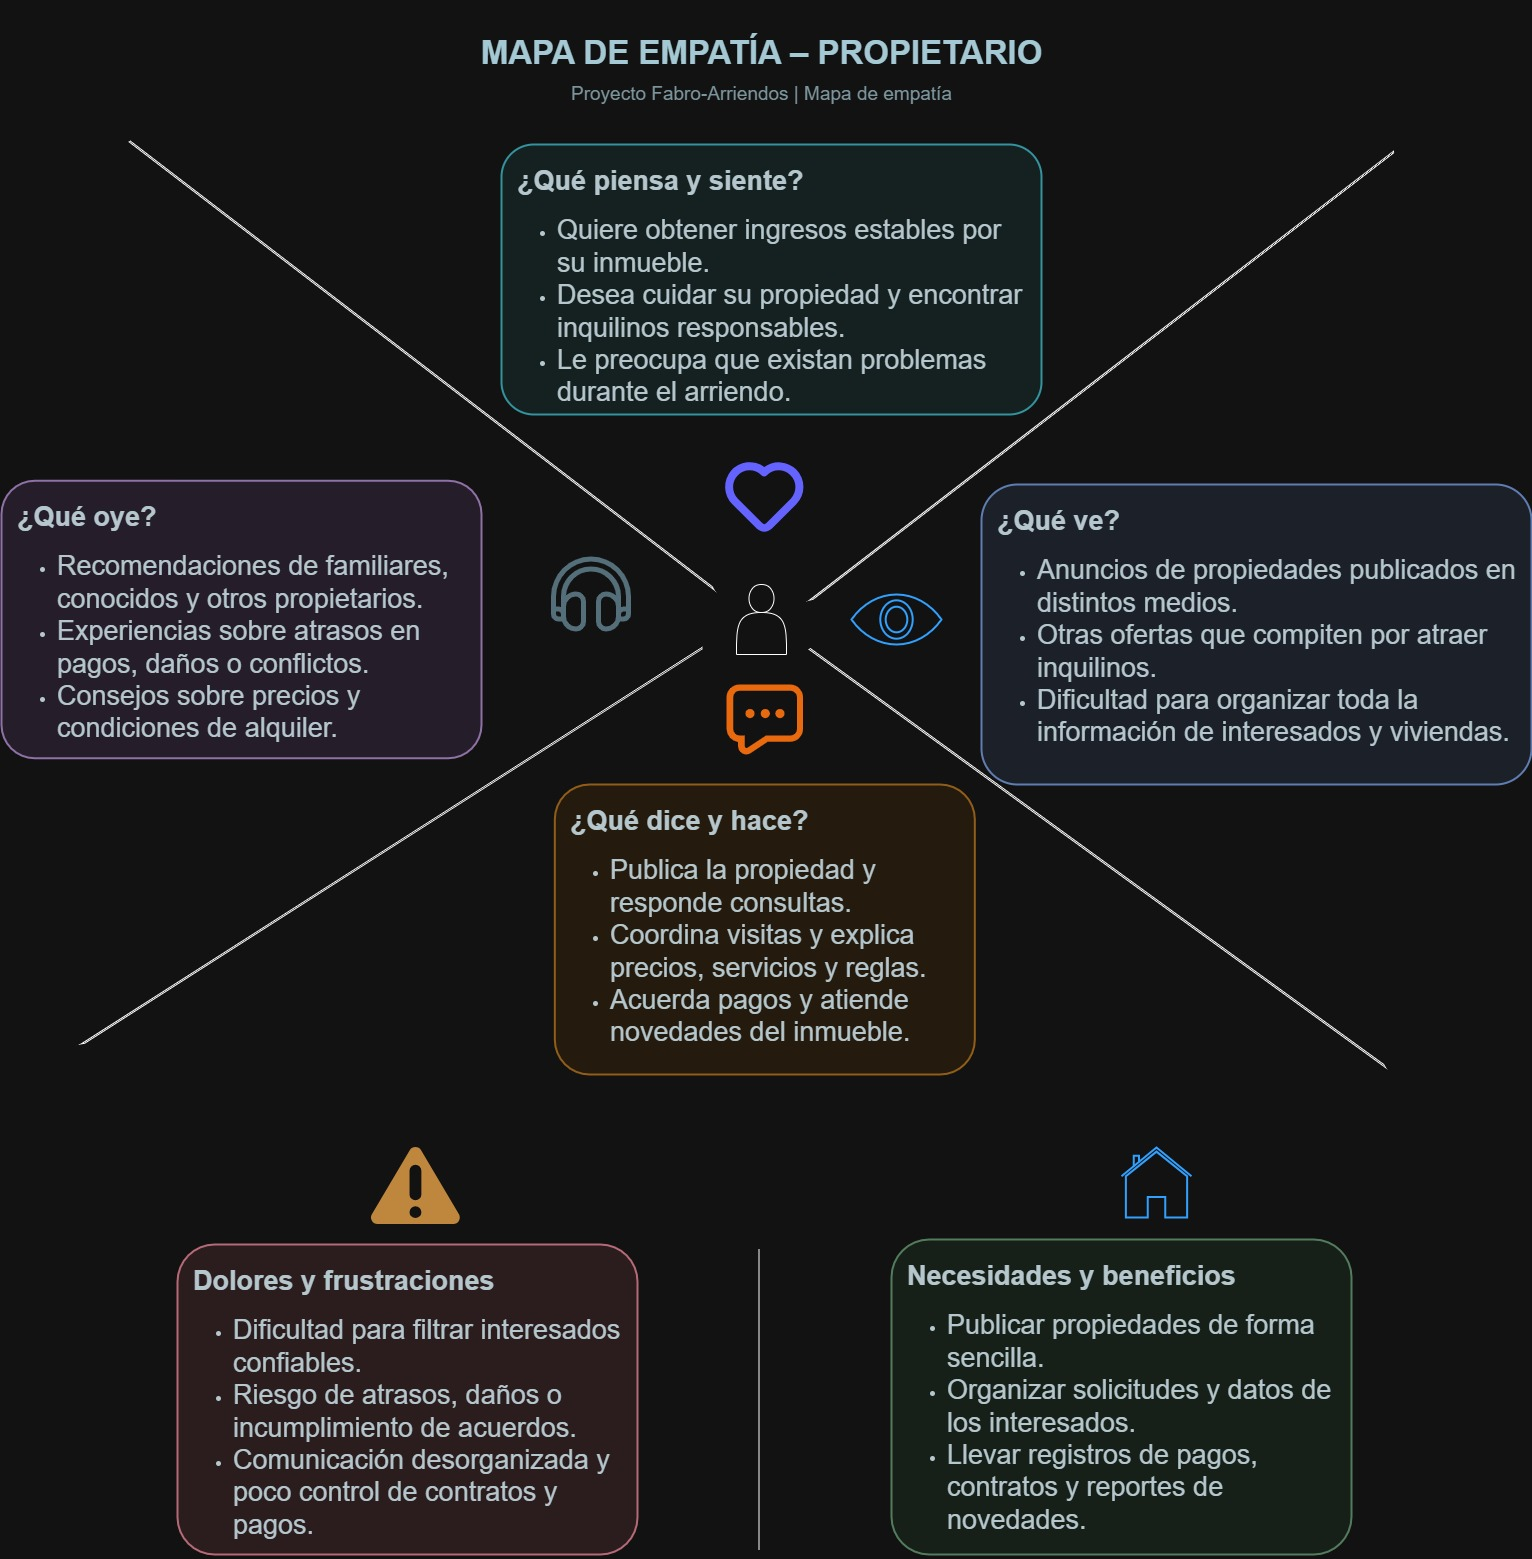
\includegraphics[width=0.78\linewidth]{figuras/mapa-empatia.jpeg}}
\caption{Mapa de empatía del propietario (Fabro-Arriendos).}
\label{fig:mapa}
\end{figure}

\subsection*{Trazabilidad del mapa con el ensayo}

``Directo'' significa que el ensayo lo dice. ``Parcial'' significa que el ensayo dice una parte. ``Inferencia'' significa que el ensayo no lo dice; es una propuesta del equipo por confirmar con propietarios reales en el trabajo de campo del PFC.

\renewcommand{\arraystretch}{1.15}
\small
\begin{longtable}{>{\raggedright\arraybackslash}p{2.2cm}>{\raggedright\arraybackslash}p{6.4cm}>{\raggedright\arraybackslash}p{2.0cm}>{\raggedright\arraybackslash}p{5.6cm}}
\caption{Trazabilidad entre el mapa de empatía y el registro del ensayo.}\label{tab:traza}\\
\toprule
\textbf{Cuadrante} & \textbf{Elemento del mapa} & \textbf{Pregunta} & \textbf{Respaldo}\\
\midrule
\endfirsthead
\toprule
\textbf{Cuadrante} & \textbf{Elemento del mapa} & \textbf{Pregunta} & \textbf{Respaldo}\\
\midrule
\endhead
Piensa y siente & Quiere ingresos estables por su inmueble & P01 & Parcial: el ensayo habla de un ingreso «extra»\\
 & Desea cuidar su propiedad y encontrar inquilinos responsables & P04, P12 & Parcial\\
 & Le preocupa que existan problemas durante el arriendo & P09, P11 & Directo\\
\midrule
Oye & Recomendaciones de familiares, conocidos y otros propietarios & P02 & Parcial: los conocidos ayudan a compartir; «otros propietarios» no aparece\\
 & Experiencias sobre atrasos, daños o conflictos & --- & Inferencia\\
 & Consejos sobre precios y condiciones & P16 & Parcial: compara lo que ve en la zona\\
\midrule
Ve & Anuncios de propiedades en distintos medios & P02 & Parcial: menciona grupos donde preguntan por cuartos\\
 & Otras ofertas que compiten por inquilinos & P16 & Parcial\\
 & Dificultad para organizar la información & P03, P05, P15 & Directo\\
\midrule
Dice y hace & Publica la propiedad y responde consultas & P02, P03 & Directo\\
 & Coordina visitas y explica precios, servicios y reglas & P03 & Directo\\
 & Acuerda pagos y atiende novedades & P03, P05, P11 & Directo\\
\midrule
Dolores & Dificultad para filtrar interesados confiables & P12 & Directo: no tiene método formal\\
 & Riesgo de atrasos, daños o incumplimiento & P08, P09, P11 & Directo\\
 & Comunicación desorganizada y poco control de contratos y pagos & P03, P05, P15 & Directo\\
\midrule
Necesidades & Publicar propiedades de forma sencilla & P02, P14 & Directo\\
 & Organizar solicitudes y datos de interesados & P03 & Directo\\
 & Llevar registros de pagos, contratos y reportes de novedades & P05, P06, P11 & Directo\\
\bottomrule
\end{longtable}
\normalsize

% =============================== PROBLEMA ===============================

\section*{5. Definición del problema}

Propuesta del equipo, por confirmar con propietarios reales.

\textbf{Usuario.} Propietario que arrienda pocos cuartos a estudiantes foráneos y los administra por su cuenta.

\textbf{Necesidad.} Saber en todo momento qué cuartos están libres, quién pagó y qué novedades hay en su inmueble, sin buscar entre mensajes, un cuaderno y una hoja de cálculo.

\textbf{Lo que se observó en el ensayo.}
\begin{itemize}
\item La información está repartida entre publicaciones, WhatsApp, un cuaderno y una hoja de cálculo que no siempre se actualiza el mismo día (P05, P15).
\item Repite las mismas respuestas a cada interesado y a veces omite un detalle, como si la luz se paga aparte (P02).
\item Puede ofrecer el mismo cuarto a dos personas porque el cuaderno no siempre está a mano (P03).
\item No sabe con exactitud cuánto gana después de gastos (P06).
\item Se entera tarde de daños y escucha versiones distintas de un conflicto (P11).
\item No tiene un método para conocer el historial de pagos de un postulante y prefiere no averiguar cosas privadas (P12).
\end{itemize}

\begin{center}
\fbox{\parbox{0.9\linewidth}{\centering\textbf{Pregunta guía:}\\[3pt]\bfseries ¿Cómo podríamos ayudar a un propietario que arrienda pocos cuartos a estudiantes a saber en todo momento qué cuartos están libres, quién ha pagado y qué ha pasado en su casa, sin depender de su memoria, un cuaderno y mensajes dispersos?}}
\end{center}

La pregunta describe la necesidad del propietario y no propone una solución. Las ideas de solución quedan para la fase de ideación.

% =============================== AJUSTES ===============================

\section*{6. Ajustes al guion}

Preguntas del ensayo que fallaron, con el defecto y su versión corregida. G indica la pregunta del guion corregido de la sección 1.

\renewcommand{\arraystretch}{1.15}
\small
\begin{longtable}{>{\raggedright\arraybackslash}p{1.0cm}>{\raggedright\arraybackslash}p{6.4cm}>{\raggedright\arraybackslash}p{3.6cm}>{\raggedright\arraybackslash}p{4.6cm}}
\caption{Preguntas defectuosas del ensayo y su corrección.}\label{tab:ajustes}\\
\toprule
\textbf{N.º} & \textbf{Pregunta del ensayo} & \textbf{Defecto} & \textbf{Versión corregida}\\
\midrule
\endfirsthead
\toprule
\textbf{N.º} & \textbf{Pregunta del ensayo} & \textbf{Defecto} & \textbf{Versión corregida}\\
\midrule
\endhead
P01 & ¿Qué te motivó a empezar a alquilar y qué espacios ofreces ahora? & Doble & G1, una sola pregunta; la motivación pasa a sondeo\\
P04 & ¿Cómo haces el acuerdo y qué cosas te parece importante dejar claras? & Doble & G4, con un sondeo\\
P05 & ¿Cómo registras quién pagó, quién se atrasó y cuánto entra cada mes? & Triple & G5, solo el registro de pagos\\
P07 & ¿Cómo cobran y dividen agua, luz e internet? & Doble & G7, solo el cobro\\
P08 & ¿Qué te pasa económicamente si alguien deja el cuarto de repente? & Hipotética y abstracta & G8, pide un caso vivido\\
P09 & ¿Qué conductas de algunos inquilinos te han causado problemas? & Pide generalizar y induce a hablar mal & G9, un caso concreto sin nombres\\
P10 & ¿Notas alguna señal cuando un inquilino piensa en irse? & Cerrada (sí o no) y presupone señales & Se retira del guion\\
P12 & ¿Cómo verificas si alguien ha tenido problemas de pago o convivencia? & Presupone que verifica y pide dos temas & G11, con «si lo hace»\\
P13 & ¿Qué medidas de seguridad tienes y qué problemas has encontrado con ellas? & Doble & G12, solo las medidas\\
P14 & ¿Qué tan difícil es conseguir otro inquilino si alguien desocupa a mitad de semestre? & Inductiva y cerrada por escala & Se retira del guion\\
P16 & ¿Cómo decides cuánto cobrar y qué hace que cambie ese precio? & Doble & G14, solo cómo decide\\
\bottomrule
\end{longtable}
\normalsize

\textbf{Notas.}
\begin{itemize}
\item Las preguntas proceden de la sección «Propietarios» del borrador del compañero Erick Alvia para el proyecto Fabro-Arriendos, que tiene 22 preguntas.
\item En el borrador, la pregunta 19 dice «nuevos propietarios». En el ensayo se interpretó como «nuevos inquilinos» (P14), porque se refiere a reemplazar a un estudiante que desocupa.
\item Tras los ajustes, el guion pasa de 16 a 14 preguntas, dentro del rango de 12 a 15 que pide la guía.
\end{itemize}

% =============================== IA ===============================

\section*{7. Declaración de uso de inteligencia artificial}

\begin{itemize}
\item \textbf{Herramienta:} Claude, de Anthropic, en su aplicación de chat. \textbf{Versión:} Claude Sonnet 5.5, según se indicaba en la interfaz.
\item \textbf{Propósito:}
  \begin{itemize}
  \item revisar el borrador de preguntas contra los criterios de pregunta abierta, neutral y simple, y proponer reformulaciones;
  \item corregir erratas del registro del ensayo, sin cambiar su contenido;
  \item armar la estructura del documento en LaTeX: inclusión de la figura, tabla de trazabilidad y tabla de ajustes;
  \item redactar un borrador de la definición del problema y del protocolo de consentimiento;
  \item sugerir puntos clave para el personaje del propietario en la simulación.
  \end{itemize}
\item \textbf{Verificación:} se compiló el documento desde cero siguiendo el \texttt{Readme.md}; se contrastó cada elemento del mapa de empatía con el texto del registro del ensayo, citando el número de pregunta; las referencias se tomaron de la guía del docente y se copiaron tal cual figuran en ella.
\item \textbf{Alcance:} la herramienta no entrevistó a nadie ni generó datos de campo. El ensayo es una simulación y está marcada como tal en todo el documento.
\end{itemize}

\bibliographystyle{IEEEtran}
\bibliography{references}

\end{document}
